\chapter{Introduction}
\section{Project Background}
In today's rapidly evolving digital landscape, cybersecurity remains a paramount concern for organizations
across all industries. With the proliferation of sophisticated cyber threats and the increasing complexity of
\acrshort{it} infrastructures, business are constantly seeking new and innovative ways to protect their
digital assets and fortify their defences and safeguard sensitive data. In this pursuit, cybersecurity
consultant firms have emerged as a critical ally for organizations, providing expert guidance and support in
the development and implementation of robust cybersecurity strategies, playing a pivotal role in offering
expertise and guidance to help organizations navigate the intricate realm of cybersecurity.

One of the key strategies employed by cybersecurity consultants is the integration of third-party security
\gls{API}s into their arsenal of tools and technologies. These \acrshort{api}s provide invaluable
functionalities, ranging from vulnerability assessment and security scans to device health monitoring and
threat intelligence analysis by \acrshort{ai}. By leveraging these \acrshort{api}s, cybersecurity consultants
can enhance their capabilities and provide a more comprehensive and effective security solution to their
clients, streamline their operations, provide clients with robust, proactive security measures, and improve
their overall service delivery.

SentinelOne emerges as one of the leading organizations in the cybersecurity real, offering cutting-edge
endpoint protection and threat intelligence solutions. It leverages advance \acrshort{ai} and \acrshort{ml}
algorithms, providing comprehensive protection against malware, ransomware, and other cyber-threats. It is one
of the must-have protection tools for business organizations looking to bolster their cybersecurity posture
and safeguard their digital assets.

As the main topic of this graduation work placement project, the author
has been tasked to integrate SentinelOne endpoint protection capabilities into the client company internal
application, the \acrshort{qaas} app. The main objective of this project is to promote transparency more
into \acrshort{qict} clients by providing them with real-time data and visibility into their organizations,
enabling them to make informed decisions and take proactive measures to protect their own digital assets and
mitigate security risks.

\section{Problem Statement}
The company currently manages numerous third-party \acrshort{api}s for the above-mentioned purposes.
Currently, the company has already offered SentinelOne endpoint protection subscription to its clients.
However, the clients cannot access to SentinelOne dashboard without \acrshort{qict} making the
necessary accounts for them first. Making the accounts for the clients can be a time-consuming process,
seeing that the clients reach up to 400 active customers, therefore an integration of SentinelOne
to \acrshort{qict}'s own internal system is more advantageous to the company by allowing clients to see
their SentinelOne data related to their system and endpoint health directly through \acrshort{qict}'s
platform. Moreover, it is not beneficial from a business perspective to direct customers to external
security solutions, as most of the data in SentinelOne is in English and \acrshort{qict} want to be the
primary resource for cybersecurity assistance for its clients around the Netherlands.

Furthermore, the SentinelOne dashboard is not user-friendly to the clients. It is made to directly assist cybersecurity
specialist like threat analysts working in \acrshort{soc} department or \acrshort{it} administrators. Therefore,
\acrshort{qict} also wishes that this integration to be designed as user-friendly as possible, considering
that most clients have limited or no knowledge at all about cybersecurity or computers. The integration of SentinelOne to the
\acrshort{qaas} App simply adds a layer of functionality and transparency to the clients, enabling them to see and easily
understand the data.

Thus, the company has tasked the author with the development of the SentinelOne security threat platform
integration for continuous cybersecurity monitoring within the \acrshort{qaas} app as the main topic of his
graduation work  placement project.

\section{Project Objectives}
In the end of this project which consist of 90-99 working days, the following objectives should be achieved:
\begin{enumerate}
      \item Effectively integrates and leverages the SentinelOne \acrshort{edr} platform for continuous
            cybersecurity monitoring within the \acrshort{qaas} app.
      \item The \acrshort{qaas} app should have a way to visualize the data retrieved from the SentinelOne
            \acrshort{api} in a user-friendly manner in order for the client users helpdesk support, financial
            department, cybersecurity department, software development department, and other employees within
            \acrshort{qict}  departments to see the data easier.
            %     \item Combine the SentinelOne data with N-Central \acrshort{api}
            %     \item Utilize Vigilance package of SentinelOne
            %     \item Ensure proper unit testing, code refactoring, commenting, and adherence to the overall code
            %           conventional guidelines and best practices in both the test and live environments of the
            %           \acrshort{qaas} app.
\end{enumerate}
Therefore, by the end of this project, SentinelOne platform will complement the \acrshort{qaas} app with the ability to
visualize and display the intricate data related to endpoint security, such as threat intelligence, endpoint
security logs, configuration details, user activity logs, telemetry data, alerts, notifications, remediation
actions, reports and analytics, \acrshort{etc}.  This project will not however, make any changes related to how
the internal system architecture of SentinelOne, including the structure of its Agents and the algorithms driven by
\acrshort{ai} and \acrshort{ml}.
\section{Reading Guide}
This report is structured as follows:
\begin{itemize}
      \item \textbf{Summary}: provides a brief and concise overview of the entire report, including the
            research questions, key findings, and conclusion. Its purpose is to provide readers with a
            quick and comprehensive understanding of the report.
      \item \textbf{Introduction}: provides an overview of the project background, the research topic of the
            company, and the project objectives. It introduces the context of the research and outlines the
            structure of the report.
      \item \textbf{Research Design}: outlines the methodologies employed during the research
            process. It describes the research approach, data collection methods, selected measuring instruments,
            data analysis techniques used to address the research questions, reliability, validity, and general
            applicability.
      \item \textbf{Research Results}: presents the research results, including the research methodology, the findings,
            and the analysis of the research questions. Firstly, it describes the methodologies employed
            during the research, and then it provides a detailed account of the research process and the
            outcomes of the research.
      \item \textbf{Realization}: provides a detailed description of the software end-product developed during
            this work placement project. It outlines insights into design, development, and implementation
            phases. It also highlights key features, functionalities, and technology specifications used in
            the project.
      \item \textbf{Conclusions and Recommendations}: the Conclusion summarizes the key findings and results
            achieved during the research and realization phases. The Recommendation section outlines the
            proposed next steps and future research areas to further enhance the project and address any
            outstanding issues. It discusses potential areas for further exploration or refinement.
      \item \textbf{References}: lists all the sources cited in the report following the appropriate to
            \acrshort{apa} 7th edition citation style.
      \item \textbf{Appendices}: includes any additional supplementary information, data, or materials that
            are relevant to the report but not included in the main body of the report.
\end{itemize}

\section{The Company}

\acrshort{qict}, is a small cybersecurity consultancy based in Emmen, northeast of the Netherlands. The company follows
a flat organizational structure, which means that there are few or no levels of middle management between the staff and
everything communication directly goes with the director. Their customers are \acrshort{sme} companies with employees ranging
from 1 to 100. \acrshort{qict} is therefore asked to monitor their clients' devices and ensuring the overall security of their
systems, \acrshort{it} infrastructure, and digital assets. As of now, \acrshort{qict} has over 400 active customers. Some notable clients
are: Kigpolis Verzekeringen, CLS Europe, and Heli Holland.

\begin{figure}[htbp]
      \centering
      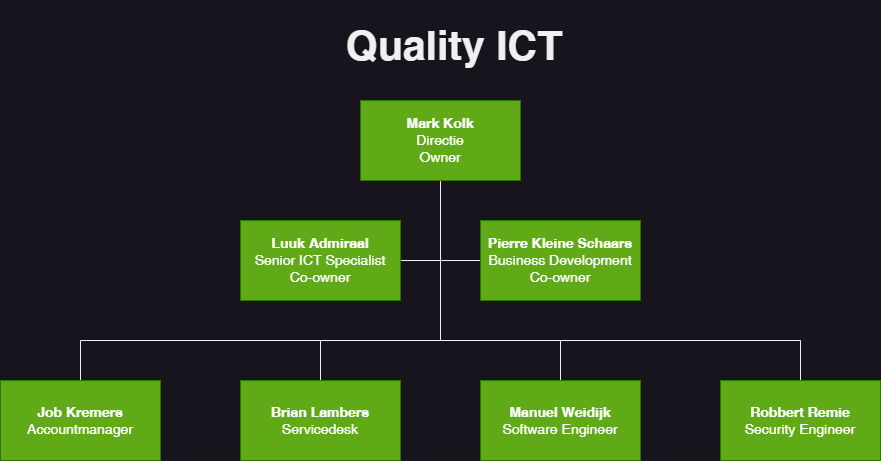
\includegraphics[width=1.0\textwidth]{Figures/OrganizationalDiagram_QICT.png}
      \caption{Flat (hierarchical) structure of \acrshort{qict}, along with its departments and their managers.}
\end{figure}

\subsubsection{Departments}

The company consists of multiple departments in its behalf, each with their own functions and responsibilities.
Those departments are the following:
\begin{enumerate}
      \item \textit{Service Help Desk Department}: it serves as a frontline support function responsible for
            addressing client inquiries, troubleshooting technical issues, and providing guidance and support
            to clients in resolving their technical challenges. It contains 2 sub-departments, the first level
            help desk and the second level help desk. The First Level Help Desk is the first point of contact
            for clients seeking technical assistance and support, and it is responsible for managing and
            resolving client issues in a timely and efficient manner. The Second Level help desk is
            responsible for providing more advanced technical support and troubleshooting for complex
            technical issues and consists of Senior System Engineers. It has 2 services, mainly the indoor
            and outdoor customer services. With the indoor customer services, the company provides remote
            support to clients, while with the outdoor customer services, the company provides on-site
            support to clients.
      \item \textit{Cybersecurity Department}: it's responsible for implementing procedures that will be used
            throughout the company's system, especially in Help Desk Department, to ensure that the company's
            information technology infrastructure is secure. It also develops methodologies and best practices
            related to cybersecurity, as well as integrating \acrshort{itil} principles and product management
            practices into the company's operations. Conducting regular security scans for clients' networks,
            systems, and applications to identify vulnerabilities and security risks and performing
            \gls{Pentest} that involves simulating cyberattacks to identify weaknesses in the client's
            defences and assess their ability to withstand and respond to real-world cyber threats. This
            department mainly consist of \acrshort{it} managers, \acrshort{pentest}ers, \acrshort{ciso}s,
            and cybersecurity specialists.
      \item \textit{Software Development Department}: it addresses \acrshort{qict} clients' need by creating
            custom software solutions tailored to their specific requirements. It consists of software
            developers that work closely with clients to understand their unique cybersecurity challenges and
            design solutions that effectively address those concerns, while utilizing their expertise in
            programming languages, software frameworks, and cybersecurity principle to develop secure and
            reliable applications. This is the department where the author is currently working on his
            graduation workplacement project. Mainly, this department uses Dart with Flutter as the main
            front-end development framework, and Node.js with TypeScript template as the main back-end
            development framework. Furthermore, it utilizes Google Firebase as the  main cloud solution for
            the applications it develops as it works together with Flutter, but it expresses its
            desires to expand more into \acrshort{ms} Azure in the future.
      \item \textit{Financial Department}: it is responsible for managing the financial aspects of the company
            to ensure its financial health and stability. It includes Accountant and Financial Advisor, and
            they are responsible for analyzing financial data, identifying trends, and making strategic
            financial decisions to support the company's growth and objectives.
\end{enumerate}

% \subsubsection{Q-ICT Sister Companies}

% \acrshort{qict} has 2 other sister companies who are also under the same ownership of Mark Kolk, which are \acrshort{mkb}iT and
% \acrshort{qaas}.nu respectively.

% \textbf{MKBiT}

% It is a parent-company of \acrshort{qict} who provides IT solutions and consultation to its clients. It was founded to support
% \acrshort{qict} business operations. It shares the same office with \acrshort{qict}. Its services include cloud solution, Microsoft 365
% products, patch-management, online-backup, \acrshort{av}, anti-spam, and monitoring software applications.

% Luuk Admiraal is directing this company. Because the company is an \acrshort{it} service provider, it has a vast network of suppliers and
% partners to provide them with the products and brands to support their business. Here is the list of the suppliers:
% DrayTek, HP, Microsoft, and Ubiquiti Network.

% \textbf{QaaS.nu}

% This company is responsible for the software development of \acrshort{qict}. It is still a small company which was set up not a while ago,
% so there is not a lot of info feasible for the author to write about it. Their upcoming projects are still proof-of-concept. The company
% is directed by Pierre Kleine Schaars. This terminology is not to be confused with the \acrshort{qaas} app, which is the internal app of
% all the three companies.

% \subsubsection{Products and Subscriptions}

% Besides cybersecurity, together with \acrshort{mkb}iT and \acrshort{qaas}.nu, \acrshort{qict} offers a wide range of products and
% services to its clients. Those products are (\textit{\cite{qictProducts}}):

% \begin{itemize}
%       \item Customized software development: this field is one of the main responsibilities of \acrshort{qict} itself, it provides
%             customers with tailor-made software solutions that are designed to meet their specific needs and requirements. The company
%             works closely with clients to understand their unique challenges and develop software applications that effectively address
%             those concerns.
%       \item Online-backup: the company offers a service where the clients can store copies of their files, documents, and data on remote
%             servers via the internet. These remote servers are hosted in secure data centres. Furthermore, \acrshort{mkb}iT also provides
%             \acrshort{db} migration in case any event of disasters occurred.
%       \item Active monitoring: the company will offer its customers the chance to oversee, track, and manage their computer systems,
%             networks, or applications in real-time. It serves various purposes, including ensuring system stability, optimizing
%             performance, enhancing security, and providing valuable insights into the usage patterns and behaviours of users or devices.
%             In the future, it wants to bring more automation to its system, providing customers with automatic messages when a disk space
%             becomes full, or when there is an error message in clients' computers.
%       \item Anti-spam software: a specific type of software application that is designed by \acrshort{mkb}iT to detect, prevent, and block
%             unsolicited and unwanted e-mail messages, commonly known as spam, from reaching clients' e-mail inboxes. They are typically
%             sent in bulk to many recipients without their consent, often containing advertisements, phishing attempts, malware, or other
%             malicious content. It has features such as whitelist, blacklist, and filter e-mails per e-mail account or e-mail address.
%       \item Microsoft 365 products: the company is also providing access to Microsoft's suite of cloud-based productivity tools and
%             services, including installation services, to its clients. These include Microsoft Word, Excel, PowerPoint, Outlook, and more,
%             which are all accessible online through a web browser or can be installed on local devices such as computers and smartphones.
%       \item \acrshort{av} software: it resells and gives clients advice and comparisons on good antivirus software from manufacturers like
%             McAfee, Bitdefender, and Kaspersky. This software is designed to detect, prevent, and remove malware from computer systems.
%       \item Cloud services: the company also provides clients with a tailor-made cloud solution based on their specific wishes and
%             problems, whether it is using a public, private, or hybrid cloud. It delivers a range of computing resources, applications,
%             and services over the internet through cloud computing technologies. These services enable the clients to access and use
%             computing resources without the need to own or maintain physical hardware and software infrastructure, enabling their
%             employees to access their files anytime, anywhere, without others having to access them.
% \end{itemize}

% In addition, for the software development, \acrshort{qict} also uses other \acrshort{ms} technologies such as Power Platform
% (\acrshort{ie} Power Automate, Power BI, Power Apps, Power Virtual Agents, and Power Pages), Dynamics 365, and Azure to help with their
% software development, therefore the clients who are asking for the product to be developed with the help of  those \acrshort{ms}
% technologies will also have those subscriptions of the products, therefore paying extra charge.

% The company also offers subscriptions, such as:

% \begin{itemize}
%       \item \acrshort{qaas} Safe:
%       \item \acrshort{qaas} Help:
%       \item \acrshort{qaas} Backup:
% \end{itemize}

% \subsubsection{Unofficial Partnerships}

% \acrshort{qict} has several unofficial partnerships with other organizations, they are normally located in the same building that
% \acrshort{qict} rents its office from. These organizations help \acrshort{qict} in their own speciality, and \acrshort{qict} helps them
% in return. These organizations are:

% \begin{itemize}
%       \item MemoICT: is a Shopware company that helps with e-commerce.
%       \item Ondernemend Emmen: helps with international entrepreneurship, knowledge sharing, and networking.
%       \item Peat Digital: helps with online marketing to promote \acrshort{qict} products more into wider audience.
%       \item Webba: helps with web development, especially designing \acrshort{qict}, \acrshort{mkb}iT, and \acrshort{qaas}.nu website.
%       \item InDiv Solutions: also helps \acrshort{qict} with the front-end side of their website development.
% \end{itemize}

\subsubsection{Working Methodology}
The company currently utilizes the five functions defined by \acrshort{nist} as part of its \acrshort{csf} as
the framework to help the company manage and improve their cybersecurity risk management processes. These five
functions are part of the \acrshort{fips} 199. All functions serve as level categories for organizing
cybersecurity activities within an organization and are as follows (\cite{nist}):
\begin{itemize}
      \item \textbf{Identify}: develop the organizational understanding to manage cybersecurity risk to
            systems, assets, data, and capabilities. This includes the development of an organizational
            understanding to manage cybersecurity risk to systems, assets, data, and capabilities. It also
            includes the development of a cybersecurity risk management strategy that is aligned with the
            organization's mission, goals, and objectives and the establishment of a governance structure to
            ensure that the strategy is effectively implemented and maintained.
      \item \textbf{Protect}: develop and implement the appropriate safeguards to ensure delivery of critical
            infrastructure services. It can help the company assists clients in implementing security controls,
            encryption mechanism, access controls, and other security measures to protect their systems and
            data from unauthorized access, disclosure, and alteration or modification.
      \item \textbf{Detect}: develop and implement the appropriate activities to identify and detect the
            occurrence of a cybersecurity event in timely manner to facilitate rapid response and mitigation
            efforts. This includes the development of a cybersecurity event detection capability that is
            integrated with the company's incident response and recovery capabilities. It will help the
            company to implement monitoring and detection mechanisms, such as intrusion detection systems,
            log analysis tools, and \acrshort{siem} systems, to detect and identify to cybersecurity incidents
            promptly.
      \item \textbf{Respond}: develop and implement the appropriate activities to act in responding
            regarding a detected cybersecurity event, containing the impact, and restoring normal operations.
            It involves activities such as developing incident response plans, conducting incident response
            drills and exercises, establishing communication channels with stakeholders, and implementing
            recovery strategies to minimize the impact of cybersecurity incidents on business operations and
            services.
      \item \textbf{Recover}: develop and implement the appropriate activities to maintain plans for
            resilience and to restore any capabilities or services that were impaired due to a cybersecurity
            incident and event, along with implementing improvements to prevent future incidents. In this
            activity,  the company should be able to develop and implement recovery plans, conduct
            post-incident reviews and analysis, identify areas for improvement, and implement measures and
            improvements to enhance resilience and prevention future incidents.
\end{itemize}

\begin{figure}[htbp]
      \centering
      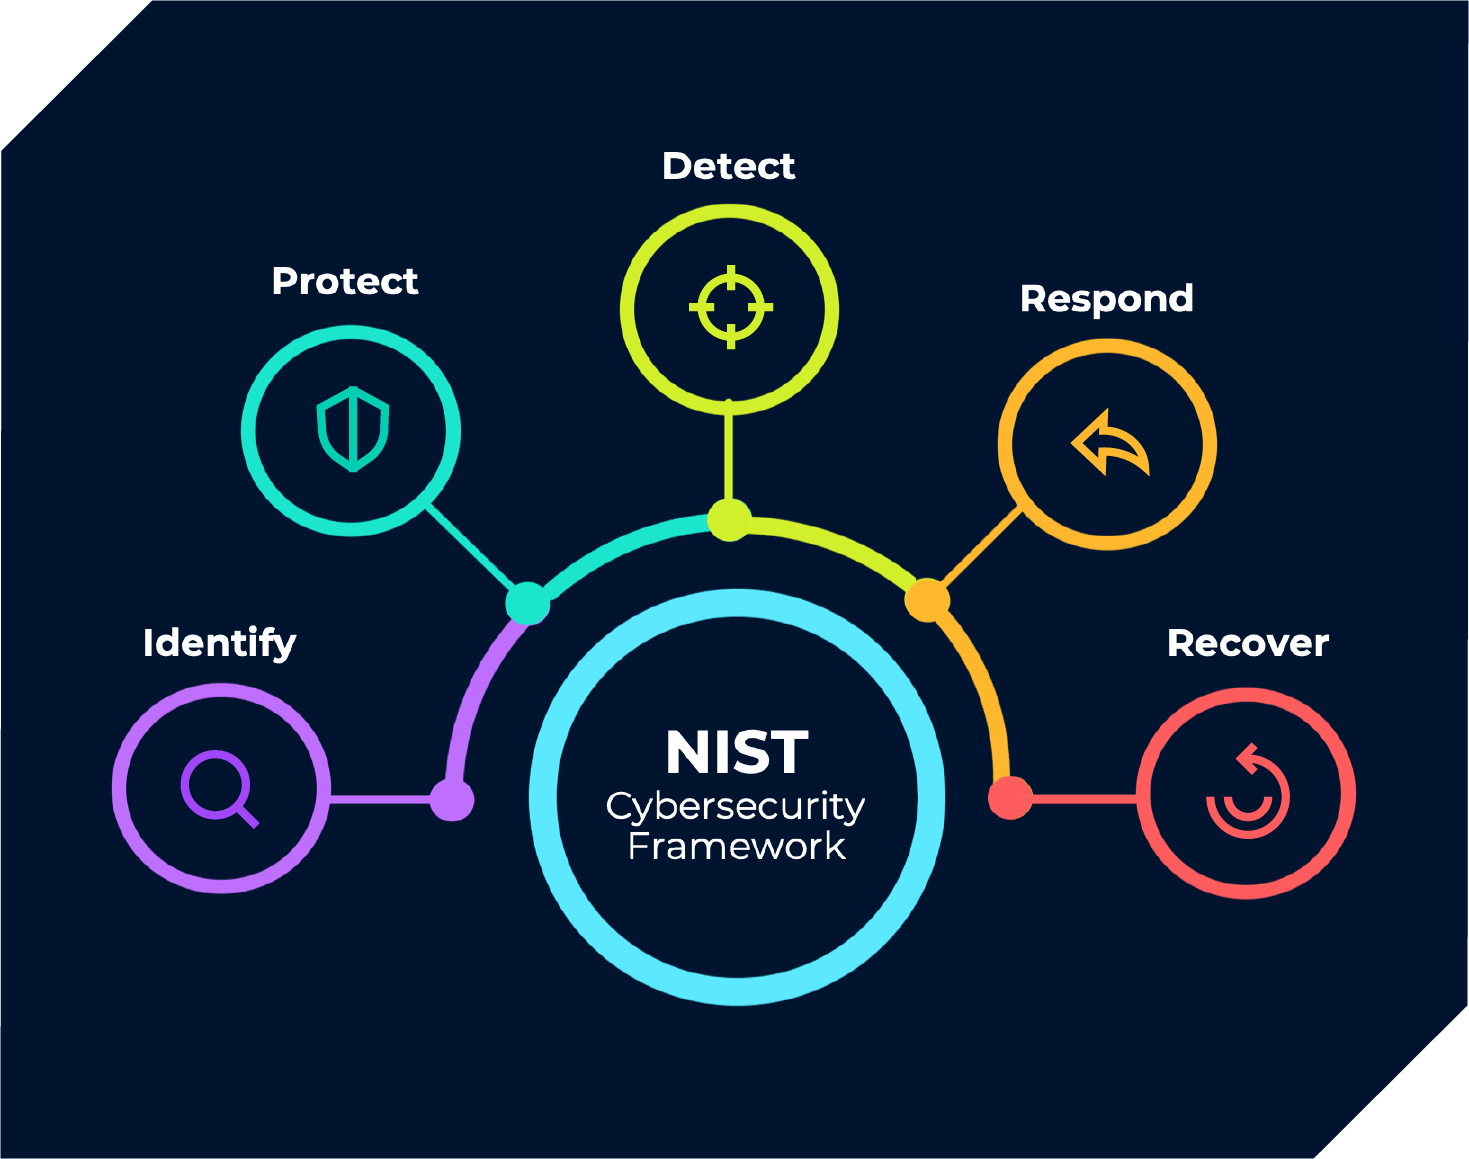
\includegraphics[width=0.8\textwidth]{Figures/qict-working-method.png}
      \caption{\acrshort{nist} working methodology that is followed by \acrshort{qict}}
\end{figure}

% \begin{figure}[htbp]
%       \centering
%       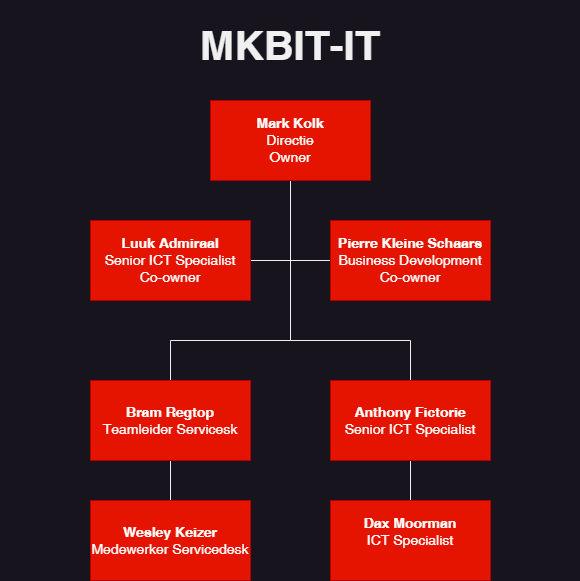
\includegraphics[width=0.8\textwidth]{Figures/Organogram-MKBiT.png}
%       \caption{Level of structure of \acrshort{mkb}iT}
% \end{figure}